%% LyX 2.0.5 created this file.  For more info, see http://www.lyx.org/.
%% Do not edit unless you really know what you are doing.
\documentclass[twocolumn,journal,cspaper,compsoc]{IEEEtran}
\usepackage[T1]{fontenc}
\usepackage{prettyref}
\usepackage{booktabs}
\usepackage{amstext}
\usepackage{graphicx}
\usepackage[unicode=true,
 bookmarks=true,bookmarksnumbered=true,bookmarksopen=true,bookmarksopenlevel=1,
 breaklinks=false,pdfborder={0 0 0},backref=false,colorlinks=false]
 {hyperref}
\hypersetup{pdftitle={A high-performance parallel radio coverage prediction tool for GRASS GIS},
 pdfauthor={Lucas Benedi\v{c}i\v{c} et al.},
 pdfpagelayout=OneColumn, pdfnewwindow=true, pdfstartview=XYZ, plainpages=false}
\usepackage{breakurl}

\makeatletter

%%%%%%%%%%%%%%%%%%%%%%%%%%%%%% LyX specific LaTeX commands.
%% Because html converters don't know tabularnewline
\providecommand{\tabularnewline}{\\}

%%%%%%%%%%%%%%%%%%%%%%%%%%%%%% User specified LaTeX commands.
% for subfigures/subtables
\ifCLASSOPTIONcompsoc
\usepackage[caption=false,font=normalsize,labelfont=sf,textfont=sf]{subfig}
\else
\usepackage[caption=false,font=footnotesize]{subfig}
\fi
%
% color tables
%
%\usepackage{colortbl}
%\definecolor{gray}{rgb}{0.9,0.9,0.9}
%
% Format of Figure cross-references
%
\usepackage{prettyref}
\newrefformat{fig}{Fig.~\ref{#1}}

\makeatother

\begin{document}
\title{A high-performance parallel radio coverage prediction tool
for GRASS GIS}

\author{Lucas~Benedi\v{c}i\v{c}, Felipe~A.~Cruz, Tsuyoshi~Hamada,~\IEEEmembership{Member,~IEEE,} and Peter~Koro\v{s}ec,~\IEEEmembership{Member,~IEEE}%

\IEEEcompsocitemizethanks{
	\IEEEcompsocthanksitem L.~Benedi\v{c}i\v{c} is with the Research and Development department, Telekom Slovenije, d.d., Cigaletova 15, SI-1000 Ljubljana, Slovenia.\protect\\
E-mail: \protect\href{mailto:lucas.benedicic@telekom.si}{lucas.benedicic@telekom.si},
see \protect\href{http://cs.ijs.si/benedicic/}{http://cs.ijs.si/benedicic/}%
	\IEEEcompsocthanksitem F.A.~Cruz and T.~Hamada are with the Nagasaki Advanced Computer Center, Nagasaki University, 1-14 Bunkyo-machi, Nagasaki-city, Nagasaki, 852-8521, Japan. E-mail: \{fcruz,~hamada\}@nacc.nagasaki-u.ac.jp,\protect\\
see \protect\href{http://nacc.nagasaki-u.ac.jp/}{http://nacc.nagasaki-u.ac.jp/}%
		\IEEEcompsocthanksitem P.~Koro\v{s}ec is with the Computer Systems department, Jo\v{z}ef Stefan Institute, Jamova cesta 39, SI-1000 Ljubljana, Slovenia.\protect\\
E-mail: \protect\href{mailto:peter.korosec@ijs.si}{peter.korosec@ijs.si},
see \protect\href{http://cs.ijs.si/korosec/}{http://cs.ijs.si/korosec/}%

}}

\markboth{IEEE Transactions on Parallel and Distributed Systems}
{Lucas~Benedi\v{c}i\v{c} \MakeLowercase{\emph{et al.}}: A high-performance parallel radio coverage prediction tool for GRASS GIS}
\IEEEcompsoctitleabstractindextext{

\begin{abstract}

We present the design and implementation of a parallel radio-coverage
prediction tool for GRASS GIS. The radio-coverage prediction problem
is used to introduce and analyze various patterns for parallel algorithm
design within the GRASS environment. Based on the serial implementation
of a similar tool, we propose a master/slave programming model for
our parallel implementation, providing an extended analysis of the
experimental results, which are based on real data from a UMTS network
currently deployed in Slovenia. According to the experiments, which
are performed on a computer cluster, the parallel radio-coverage prediction
tool has very good scalability properties, meaning it is able to calculate
the radio-coverage prediction of real-world networks while greatly
reducing processing time and maximizing performance. Moreover, we
are able to solve problem instances, which sizes are out of reach
of the reference serial implementation.

\end{abstract}

\begin{keywords}

Mobile networks, GSM, UMTS, LTE, parallel, coverage, simulation, GRASS,
GIS, MPI.

\end{keywords}

}
\maketitle

\IEEEpubid{\makebox[\columnwidth]{\hfill 0000--0000/00/\$00.00~\copyright~2012 IEEE}
\hspace{\columnsep}\makebox[\columnwidth]{Published by the IEEE Computer Society\hfill}\IEEEpubidadjcol}


\section{Introduction}

\PARstart{M}{ore} than 20 years have passed since the world's first
GSM mobile call was made in Finland. Still, the coverage planning
of the radio network remains a key problem that all mobile operators
have to deal with. Moreover, it has proven to be a fundamental issue
not only in GSM networks, but also in modern standards such as the
third generation (3G) UMTS and the fourth generation (4G) LTE Advanced
\cite{Saleh_On_the_coveraga_extension_in_LTE_networks:2010,Shabbir_Comparison_of_radio_propagation_models:2011,Siomina:Minimum.pilot.power.for.service.coverage,Valcarce_Applying.FDTD.to.the.coverage.prediction.of.WiMAX:2009}.
In radio networks is generally the case that the radio stations are
installed at fixed locations. For this reason, one of the primary
objectives of mobile-network planning is to efficiently use the allocated
frequency band to assure that the whole of the geographic area of
interest can be satisfactorily reached with the radio stations of
the network. To this end, radio-coverage prediction tools are of great
importance as it allows the network engineers to test different network
configurations before physically implementing the changes. Nevertheless,
radio-coverage prediction is a complex task due to the wide range
of various combinations of hardware and configuration parameters which
have to be analyzed in the context of different environments. The
complexity of the problem means that radio-coverage prediction can
be a computationally-intensive and time-consuming task, hence the
importance of fast and accurate prediction tools.

Although different mathematical models have been proposed for radio
propagation modeling, none of them excels in a network-wide scenario
\cite{Shabbir_Comparison_of_radio_propagation_models:2011}. A combination
of different models and parameters is generally needed in order to
calculate radio-propagation predictions for particular environments.
Moreover, since the number of deployed cells (transmitters) keeps
growing with the adoption of modern standards \cite{Saleh_On_the_coveraga_extension_in_LTE_networks:2010},
there is a clear need for a radio propagation tool that is able to
cope with larger work loads in a feasible amount of time.

Despite various options of commercial tools specialized in radio-propagation
modeling, the common thread among them is the restricted nature of
its usage, mostly dominated by black-box implementations. This fact
induces lack of adaptability, sometimes even combined with cumbersome
user interfaces that are not suitable for big batch jobs, involving
thousands of transmitters. Moreover, the evolution of any commercial
tool is strictly bounded to its vendor, forcing the user to adapt
its work-flow to it, when the opposite situation should be preferred.

To tackle the afore-mentioned issues, we present a high-performance
parallel radio-prediction tool for the open source Geographic Resources
Analysis Support System (GRASS). For its design, we have focused on
scalability, clean design and open nature of the tool, inspired by
the GRASS geographic information system (GIS). These facts make it
an ideal candidate for calculating radio-predictions of big problem
instances, i.e. real mobile networks containing thousands of transmitters.
This is also true for the scientific research community, since our
design may be used as a template for parallelization of computationally-expensive
tasks within the GRASS environment.


\subsection{Parallel computation on computer clusters}

In consideration of the high computational-intensity of predicting
the radio-coverage of a real mobile network, the use of a computer
cluster is required, i.e. a group of interconnected computers that
work together as a single system. To reach high levels of parallel
performance and scalability, this work discusses in detail the key
steps of parallel decomposition of the radio-coverage prediction problem
for real networks and the distribution of the computational load among
the computing nodes that belong to the cluster.

Such computer clusters typically consist of several commodity PCs
connected through a high-speed local network with a distributed file
system, like NFS \cite{Shepler_Network_file_system:2003}. One such
system is the DEGIMA cluster \cite{Hamada_Cluster_of_GPUs:2010} at
the Nagasaki Advanced Computing Center of the Nagasaki University.
This system ranked in the TOP 500 list of supercomputers until June
2012%
\footnote{http://www.top500.org%
}, and in June 2011 held the third place of the Green 500 list%
\footnote{http://www.green500.org%
} as one of the most energy-efficient supercomputers in the world.




\subsection{Objectives\label{sub:Objectives}}

The main goal of this work is to develop a radio prediction tool to
be used in large real-world network environments, such as the ones
currently deployed by several mobile operators around the world. To
achieve this, we have developed a high-performance parallel radio
prediction tool (PRATO) for radio networks. Therefore, our focus is
on the performance and scalability of PRATO, while other more dynamic
aspects of radio networks are not considered. Among these aspects
are code distributions, details of (soft) handover, and dynamics related
to radio resource management.



The performance evaluation of PRATO in a distributed computing environment
is a major objective of this work. Furthermore, by presenting a detailed
description of the design and implementation of the parallel version
of PRATO, we intend to provide guidelines on how to achieve high efficiency
levels of task parallelization in GRASS GIS. Additionally, we introduce
techniques to overcome several obstacles encountered during our research
as well as in related work, which significantly improve the quality
and performance of the presented implementation, e.g. the inability
to use GRASS in a threaded environment, lowering overhead of I/O operations,
saving simulation results asynchronously and independently from GRASS,
and improving load balancing with a new message-passing technique.



The paper is organized as follows. Section \ref{sec:Description-of-the-radio-coverage-prediction-tool}
gives a description of the radio prediction tool, including the propagation
model and GRASS GIS. Section \ref{sec:Design-and-implementation}
concentrates on the design principles and implementation details of
the radio propagation tool, for the serial and parallel versions.
Section \ref{sec:Simulations} discusses the experimental results
and their analysis. Finally, Section \ref{sec:Related-work} gives
an overview of relevant publications, describing how they relate to
our work, before drawing some conclusions.


\section{Description of the radio coverage prediction tool \label{sec:Description-of-the-radio-coverage-prediction-tool}}

PRATO is a high-performance radio-prediction tool for GSM (2G), UMTS
(3G) and LTE (4G) radio networks. It is implemented as a module for
the GRASS Geographical Information System (for details of GRASS see
Section \ref{sub:GRASS-GIS}). It can be used for planning the different
phases of a new radio-network installation, as well as a support tool
for maintenance activities related to network troubleshooting or upgrading. 

As a reference implementation, we have used the publicly available
radio coverage prediction tool, developed by Hrovat et al. \cite{Ozimek_Open.source.radio.coverage.prediction:2010}.
The authors of this work have developed a modular radio coverage tool
that performs separate calculations for radio-signal path loss and
antenna radiation patterns, also taking into account different configuration
parameters, such as antenna tilting, azimuth and height. The output
result, saved as a raster map, is the maximum signal level over the
target area, in which each point represents the received signal from
the best serving cell (transmitter). This work implements some well-known
radio propagation models, e.g. Okumura-Hata and COST 231, the later
is explained in more detail in Section \ref{sub:COST-231-model}.
Regarding the accuracy of the predicted values, the authors report
comparable results to those of a state-of-the-art commercial tool.
Therefore, we use the implementation developed by \cite{Ozimek_Open.source.radio.coverage.prediction:2010}
as the reference implementation for PRATO. Furthermore, to ensure
that our implementation is completely compliant with the afore-mentioned
reference, we have designed a comparison test that consists of running
both the reference and PRATO with the same input parameters. The test
results from PRATO and the reference implementation are identical.


\subsection{Propagation modeling\label{sub:COST-231-model}}

The COST-231 Walfisch-Ikegami radio-propagation model was introduced
as an extension of the well-known COST Hata model \cite{Shabbir_Comparison_of_radio_propagation_models:2011,Sarkar_Survey_of_radio_propagation_models:2003},
designed for frequencies above 2000~MHz. The suitability of this
model comes from the fact that it distinguishes between line-of-sight
(LOS) and non-line-of-sight (NLOS) conditions. Equation (\ref{eq:cost231_LOS})
describes the path loss when there is LOS between the transmitter
and the receiver.
\begin{equation}
PL_{\textrm{LOS}}(d)=42.64+26\log(d)+20\log(F),\label{eq:cost231_LOS}
\end{equation}
where $d$ is the distance (in kilometers) from the transmitter to
the receiver point, and $F$ is the frequency, expressed in MHz.

On the other hand, in NLOS conditions, the path loss is calculated
as

\begin{equation}
PL_{\textrm{NLOS}}(d)=L_{0}+L_{\textrm{RTS}}+L_{\textrm{MSD}},\label{eq:cost231_NLOS}
\end{equation}
where $L_{0}$ is the attenuation in free space, $L_{\textrm{RTS}}$
represents the diffraction from roof top to street, and $L_{\textrm{MSD}}$
represents the diffraction loss due to multiple obstacles.

In this work, as well as in the reference implementation \cite{Ozimek_Open.source.radio.coverage.prediction:2010},
the terrain profile is used for LOS determination. The wave-guide
effect in streets of big cities is not taken into account, because
the building data is not available. In order to compensate the missing
data, we include a correction factor, based on the land usage (clutter
data). This technique is also adopted by other propagation models
for radio networks, like the artificial neural networks macro-cell
model developed by Neskovic et al. \cite{Neskovic_Microcell_electric_field_strength_prediction_model:2010}.
Consequently, both Equations (\ref{eq:cost231_LOS}) and (\ref{eq:cost231_NLOS})
have an extra term for signal loss due to clutter ($L_{\textrm{CLUT}}$),
thus redefining the LOS and NLOS path losses as

\begin{equation}
PL_{\textrm{LOS}}(d)=42.64+26\log(d)+20\log(F)+L_{\textrm{CLUT}}\label{eq:cost231_LOS-1}
\end{equation}
and

\begin{equation}
PL_{\textrm{NLOS}}(d)=L_{0}+L_{\textrm{RTS}}+L_{\textrm{MSD}}+L_{\textrm{CLUT}}.\label{eq:cost231_NLOS-1}
\end{equation}



\subsection{GRASS Geographical Information System\label{sub:GRASS-GIS}}

As the software environment for PRATO we have chosen GRASS (Geographic
Resources Analysis Support System) \cite{neteler2002:GRASS_GIS},
which is a free and open-source software project that implements a
Geographical Information System (GIS). This GIS software was originally
developed at the US Army Construction Engineering Research Laboratories
and is a full-featured system with a wide range of analytical, data-management,
and visualization capabilities. Currently, the development of GRASS
GIS is supported by a growing community of volunteer developers.

The use of GRASS GIS as an environment for PRATO presents many advantages.
First, the current development of GRASS is primarily Linux-based.
Since the field of high performance computing is dominated by Linux
and UNIX systems, an environment with Linux support is critical for
this work. Software licensing is another important consideration for
choosing GRASS, since it is licensed under the GNU Public License
\cite{Stallman_GNU_License:1991} and imposes the availability of
the source code. This allows us to make potential modifications to
the system, thus adapting it for the parallel computation environment.
Moreover, being an open system, GRASS provided us with a great deal
of useful built-in functionality, capable of operating with raster
and vector topological data that can be stored in an internal format
or a relational database. For additional information about the GRASS,
we refer the reader to the numerous guides and tutorials available
online.


\section{Design and implementation \label{sec:Design-and-implementation}}

\begin{figure}[tbh]
\centering

\includegraphics[width=0.67\columnwidth]{img/serial_implementation_flow_diagram}

\caption{\textit{\emph{Flow diagram of the serial version.}}\textit{\label{fig:serial_version_flow_diagram}}}
\end{figure}


\begin{figure*}[tbh]
\begin{minipage}[t]{0.49\textwidth}%
\centering

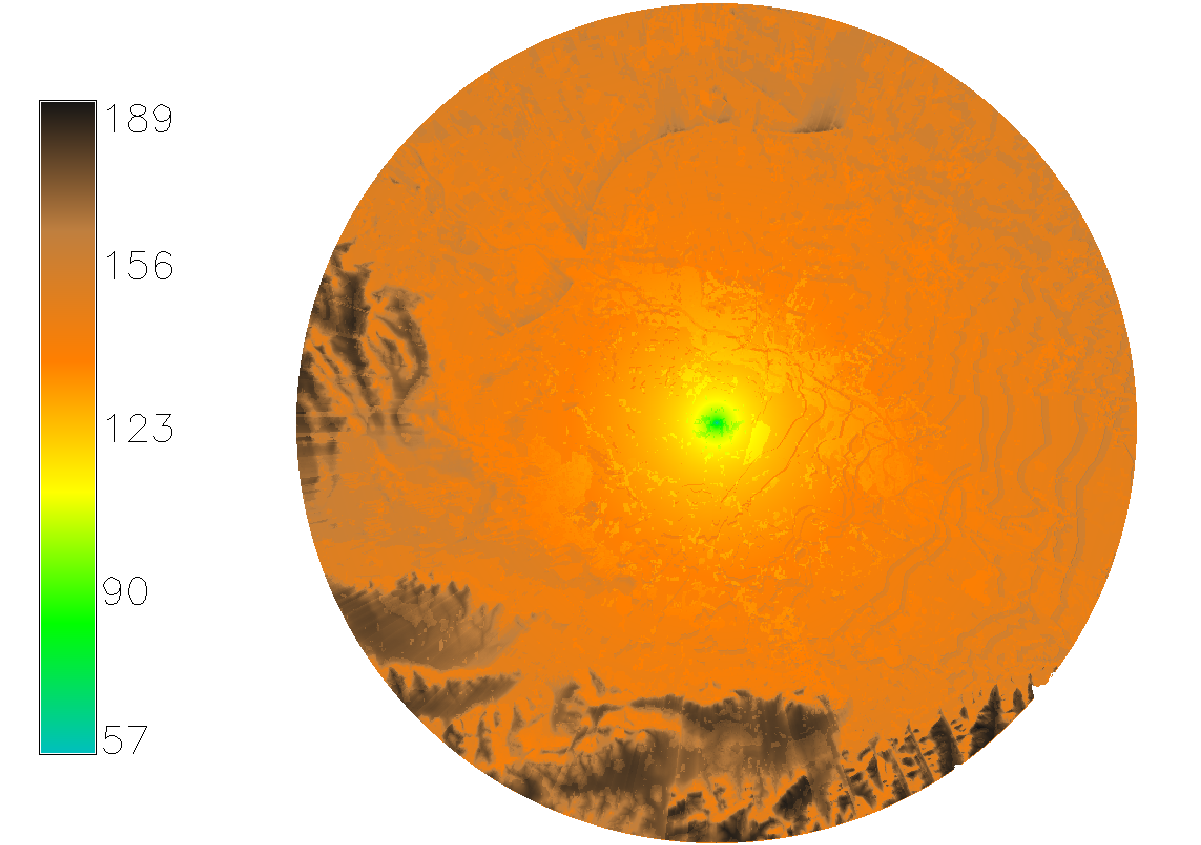
\includegraphics[width=0.8\columnwidth]{img/isotrophic_calculation}

\caption{\textit{\emph{Example of raster map, showing the result of a path-loss
calculation from an isotropic source.\label{fig:path_loss-example}}}}
%
\end{minipage}\hfill{}%
\begin{minipage}[t]{0.49\textwidth}%
\centering

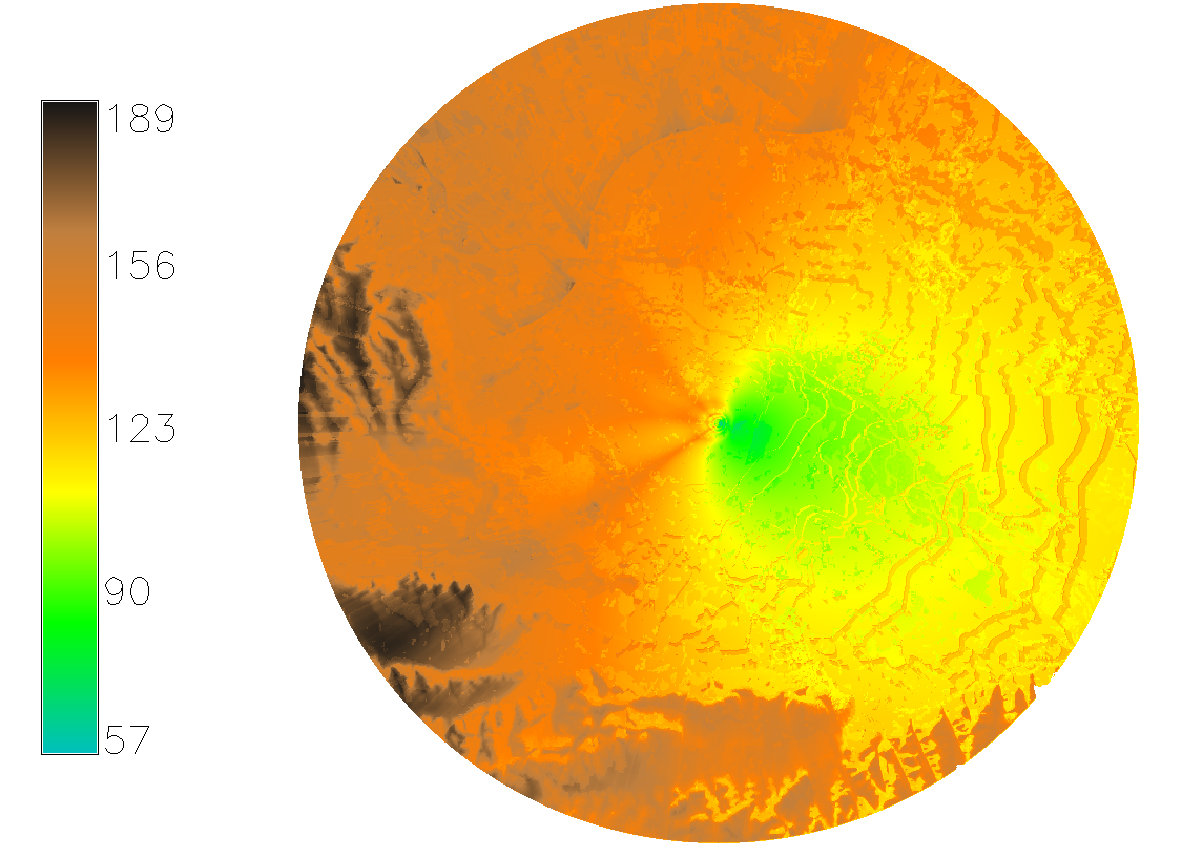
\includegraphics[width=0.8\columnwidth]{img/antenna_calculation}

\caption{\textit{\emph{Example of raster map, showing the antenna influence
over the isotropic path-loss result.\label{fig:antenna-example}}}}
%
\end{minipage}
\end{figure*}



\subsection{Design of the serial version}

This section describes the different functions contained in the serial
version of PRATO, which is implemented as a GRASS module. Their connections
and data flow are depicted in \prettyref{fig:serial_version_flow_diagram},
where the parallelograms in the flow diagram represent input/output
(I/O) operations. 

Our design follows a similar internal organization as the radio planning
tool developed by Hrovat et al. \cite{Ozimek_Open.source.radio.coverage.prediction:2010},
but with some essential differences. Specifically, we have decided
to avoid the modular design to prevent the overhead of I/O operations
for communicating data between the components of the modular architecture.
Instead, we have chosen a monolithic design, in which all the steps
for generating the radio coverage prediction are calculated inside
one GRASS module. Regarding the way results are saved, our approach
employs a direct connection to an external database server, instead
of the slow built-in GRASS database drivers. To explicitly avoid tight
coupling with a specific database vendor, the generated output is
formatted in plain text, which is then forwarded to the database server.
Any further processing is achieved by issuing a query over the database
tables that contain the partial results for each of the processed
transmitters.


\subsubsection{Read input parameters\label{sub:Read-input-parameters}}

All input data are read in the first step (see ``Read input data''
in \prettyref{fig:serial_version_flow_diagram}), e.g. digital elevation
model, clutter data, transmitter configurations, and other service-dependent
settings. Their format differs based on the data they contain, namely:
\begin{itemize}
\item GRASS raster files are used for the digital elevation model and clutter
data, whereas
\item a text file is used for the transmitter configurations and other simulation-dependent
options.
\end{itemize}
Since the module accepts a considerable amount of input parameters,
they are read from a text-based initialization (INI) file. This is
far more practical than passing them as command-line parameters, which
would make them error-prune and difficult to read. Besides, the INI
file may contain configuration parameters for many transmitters. The
user selects which one(s) to use at run-time by passing a command-line
option.


\subsubsection{Isotropic path-loss calculation\label{sub:Path-loss-for-isotrophic-source}}

The first step here is to calculate which receiver points, $r$, are
within the specified transmission radius (see ``transmission radius''
in \prettyref{fig:serial_version_flow_diagram}). For these points,
the LOS and NLOS conditions are calculated, with respect to the transmitter
(see ``Calculate LOS/NLOS'' in \prettyref{fig:serial_version_flow_diagram}).
The following step consists of calculating the path loss for an isotropic
source (or omni antenna). This calculation is performed by applying
the COST-231 path-loss model, which was previously introduced in Section
\ref{sub:COST-231-model}, to each of the points within the transmission
radius around the transmitter. Depending on whether the receiver point
$r$ is in LOS or NLOS, either Equation~(\ref{eq:cost231_LOS-1})
or Equation~(\ref{eq:cost231_NLOS-1}) is respectively applied (see
``Apply COST-231, LOS'' or ``Apply COST-231, NLOS'' in \prettyref{fig:serial_version_flow_diagram}).

\prettyref{fig:path_loss-example} shows a portion of a raster map
with an example result of the isotropic path-loss calculation. The
color scale is given in dB, indicating the signal loss from the isotropic
source, located in the center. Also, the hilly terrain is clearly
distinguished due to LOS and NLOS conditions from the signal source.


\subsubsection{Antenna diagram influence\label{sub:Antenna-diagram-influence}}

This step considers the antenna radiation diagram of the current transmitter
and its influence over the isotropic path-loss calculation (see ``Calculate
antenna influence'' in \prettyref{fig:serial_version_flow_diagram}).
Working on the in-memory results generated by the previous step, the
radiation diagram of the antenna is taken into account, including
beam direction, electrical and mechanical tilt. \prettyref{fig:antenna-example}
shows a portion of a raster map, where this calculation step has been
applied to the results from \prettyref{fig:path_loss-example}. Notice
the distortion of the signal propagation that the antenna has introduced.


\subsubsection{Transmitter path-loss prediction\label{sub:Transmitter-path-loss-prediction}}

In this step, the coverage prediction of the transmitter is saved
in its own database table (see ``Save transmitter path-loss to DB''
in \prettyref{fig:serial_version_flow_diagram}), thus considerably
enhancing the write performance during the result-dumping phase, which
involves saving the path-loss results. This is accomplished by connecting
the standard output of the developed module with the standard input
of a database client. Naturally, the generated plain text should be
understood by the database server itself.


\subsubsection{Coverage prediction\label{sub:Final-coverage-prediction}}

The final radio coverage prediction, containing an aggregation of
the partial path-loss predictions of the involved transmitters, is
created in this step (see ``Create final coverage prediction'' in
\prettyref{fig:serial_version_flow_diagram}). The received signal
strength from each of the transmitters is calculated as the difference
between its transmit power and path loss for the receiver's corresponding
position. This is done for each point in the target area by executing
an SQL query over the tables containing the path-loss predictions
of each of the processed transmitters.

Finally, the output raster is generated, using the GRASS built-in
modules $v.in.ascii$ and $v.to.rast$, which create a raster map
using the results of the above-mentioned query as input. The raster
map contains the maximum received signal strength for each individual
point, as shown in \prettyref{fig:output_raster_example}. In this
case, the color scale is given in dBm, indicating the received signal
strength from the transmitters.

\begin{figure}[tbh]
\centering

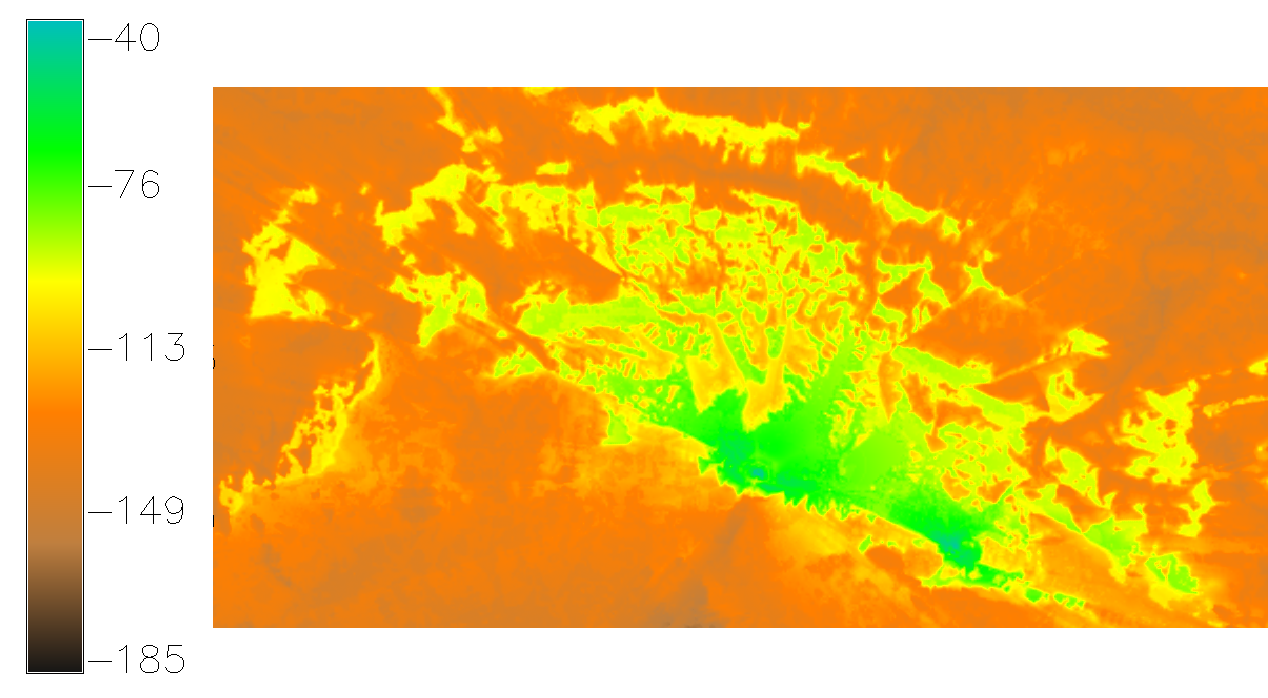
\includegraphics[width=0.95\columnwidth]{img/final_coverage}

\caption{\textit{\emph{Example of raster map, displaying the final coverage
prediction of several transmitters. The color scale is given in dBm,
indicating the received signal strength.\label{fig:output_raster_example}}}}
\end{figure}



\subsection{Multi-paradigm parallel programming}

The implementation methodology adopted for PRATO follows a multi-paradigm
parallel programming approach in order to fully use the resources
of a computing cluster. To effectively use a shared memory multi-processor,
PRATO uses POSIX threads to implement parallelism \cite{Butenhof_Programming.with.POSIX.threads:1997}.
In a nutshell, POSIX thread is a POSIX standard for creating and manipulating
light-weight processes or threads. By using POSIX threads, multiple
threads can exist within the same process while sharing its resources.
For instance, an application using POSIX threads can execute multiple
threads in parallel by using the cores of a multi-core processor,
or use the system resources more effectively, thus avoiding process
execution-halt due to I/O latency by using one thread for computing
while a second thread waits for an I/O operation to complete. 

To use the computing resources of a distributed memory system, such
as a cluster of processors, PRATO uses the Message Passing Interface
(MPI) \cite{Gropp_Using_MPI:1999}. MPI is a message-passing standard
which defines syntax and semantics designed to function on a wide
variety of parallel computers. MPI enables multiple processes running
on different processors of a computer cluster to communicate with
each other. MPI was designed for high performance on both massively
parallel machines and on workstation clusters. It has been developed
by a broadly based committee of vendors, developers, and users.

In order to make the text more clear and to differentiate between
the programming paradigms used from here on, we will refer to a POSIX
thread simply as a `thread' and a MPI proccess as a `process'.


\subsection{Design of the parallel version\label{sub:Design-parallel}}

Keeping our focus on the performance of PRATO, we are introducing
a new distributed implementation to overcome computational-time constraints
that prevented the reference implementation from tackling big problem
instances \cite{Ozimek_Open.source.radio.coverage.prediction:2010}.

Some authors have already published their work on implementing parallel
versions of GRASS modules for solving different time-consuming tasks
\cite{Akhter_Porting_GRASS_raster_module_to_distributed_computing:2007,Campos_Parallel_modelling_in_GIS:2012,Sorokine_Parallel_visualization_in_GRASS:2007}.
However, one major drawback of GRASS as a parallelization environment
is that it is not thread-safe, meaning that concurrent changes to
a data set have undefined behavior. To overcome this problem, we present
a technique that saves the simulation results asynchronously and independently
from the GRASS environment, e.g. into an external database system.
This database system works also as an input source, serving data to
GRASS, whether it is used to aggregate the partial results of the
path-loss prediction or to visualize them. We also introduce a methodology
that allows the parallel implementation to be almost completely GRASS
independent. This means that a GRASS installation is needed on only
one of the nodes, i.e. the master node of the target computer cluster.
Also, a message-passing technique is proposed to distribute the work-load
among nodes hosting the worker processes. Using this technique, computing
nodes featuring more capable hardware receive more work than those
with weaker configurations, thus ensuring a better utilization of
the available computing resources despite hardware diversity.


\subsubsection{Master process\label{sub:Master-process}}

As it has been suggested before, the parallel version of PRATO follows
a master-worker model. The master process, for which the flow diagram
is given in \prettyref{fig:master_process}, is the only component
that should be run from within the GRASS environment. As soon as the
master process starts, the input parameters are read. This step corresponds
to ``Read input data'' in \prettyref{fig:master_process}, and it
is done in a similar way as in the serial version. In the next step,
the master process dynamically initiates the worker processes using
the available computing nodes (see ``Dynamic worker-process spawning''
in \prettyref{fig:master_process}), based on the amount of transmitters
for which the coverage prediction should be calculated. In other words,
this means that master process never starts more worker processes
than there are transmitters to be processed. However, most often is
the number of transmitters larger than the amount of available computing
nodes. Therefore, the master process can assign several transmitters
to each of the worker processes. For distributing the work among the
worker processes, the master process proceeds to decompose the loaded
raster data into arrays of basic-data-type elements, e.g. floats or
doubles, before dispatching them to the multiple worker processes
(see ``Input data broadcasting'' in \prettyref{fig:master_process}).
The decomposition of the data applies to the digital-elevation and
the clutter data only. In the next step, the master process starts
a message-driven processing loop (see ``Processing loop'' in \prettyref{fig:master_process}),
which main task is to assign and distribute the configuration data
of different transmitters among idle worker processes.

\begin{figure}[tbh]
\centering

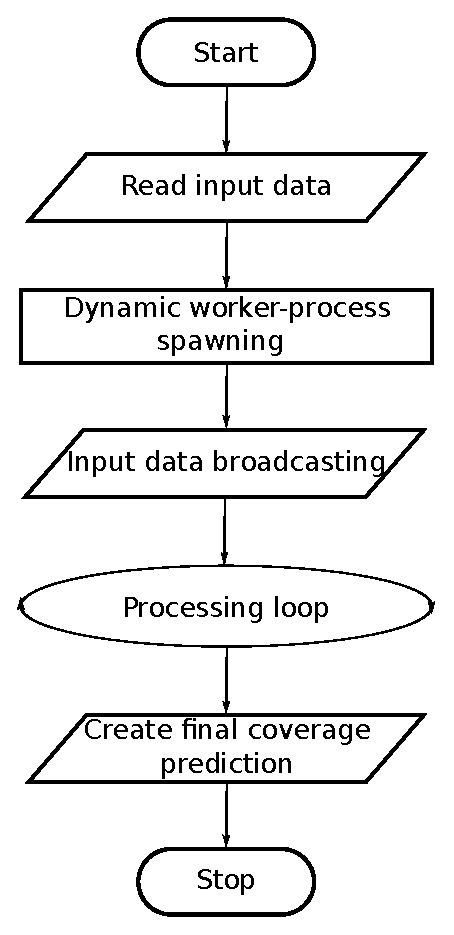
\includegraphics[width=0.4\columnwidth]{img/master_process_flow_diagram}

\caption{\textit{\emph{Flow diagram of the master process.\label{fig:master_process}}}}
\end{figure}


The flow diagram shown in \prettyref{fig:processing_loop_in_master_process}
depicts in more detail the steps inside the ``Processing loop''
step of the master process. In the processing loop, the master process
starts by checking the available worker processes, which will calculate
the radio coverage prediction for the next transmitter. It is worth
pointing out that this step also serves as a stopping condition for
the processing loop itself (see ``Any worker still on?'' in \prettyref{fig:processing_loop_in_master_process}).
The active worker processes inform the master process they are ready
to compute by sending an idle message (see ``Wait for idle worker''
in \prettyref{fig:processing_loop_in_master_process}). The master
process then announces the idle worker process it is about to receive
new data for the next calculation, and it dispatches the complete
configuration of the transmitter to be processed (see ``Send keep-alive
message'' and ``Send transmitter data'' steps, respectively, in
\prettyref{fig:processing_loop_in_master_process}). This is only
done in case there are transmitters for which the coverage prediction
has yet to be calculated (see ``Any transmitters left?'' in \prettyref{fig:processing_loop_in_master_process}).
The processing loop of the master process continues to distribute
transmitter data among worker processes, which asynchronously become
idle as they finish the coverage-prediction calculations for the transmitters
they have been assigned by the master process. When there are no more
transmitters left, all the worker processes announcing they are idle
will receive a shutdown message from the master process, indicating
them to stop running (see ``Send stop message'' in \prettyref{fig:processing_loop_in_master_process}).
The master process will keep doing this until all worker processes
have finished (see ``Any worker still on?'' in \prettyref{fig:processing_loop_in_master_process}),
thus fulfilling the stopping condition of the processing loop.

\begin{figure}[tbh]
\centering

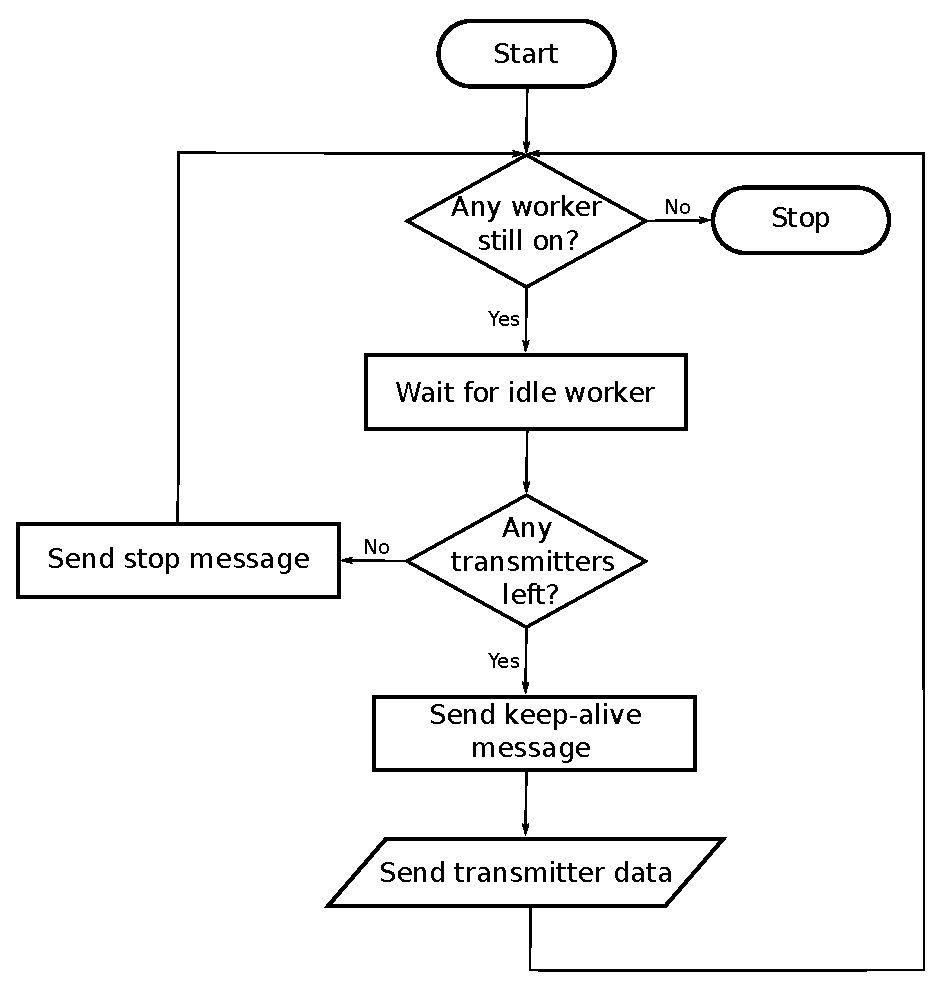
\includegraphics[width=0.85\columnwidth]{img/master_processing_loop_flow_diagram}

\caption{\textit{\emph{Flow diagram of the ``Processing loop'' step of the
master process.\label{fig:processing_loop_in_master_process}}}}
\end{figure}


Finally, the last step of the master process is devoted to creating
the final output of the calculation, e.g. a raster map (see ``Create
final coverage prediction'' in \prettyref{fig:master_process}).
The final coverage prediction of all transmitters is an aggregation
from the individual path-loss results created by each of the worker
processes during the ``Processing loop'' phase in \prettyref{fig:master_process},
which provides the source data for the final raster map. The aggregation
of the individual transmitter path-loss results is accomplished in
a similar way as in the serial version.


\subsubsection{Worker processes}

An essential characteristic of the worker processes is that they are
completely independent from GRASS, i.e. they do not have to run within
the GRASS environment nor use any of the GRASS libraries to work.
This aspect significantly simplifies the deployment phase to run PRATO
on a computer cluster, since no GRASS installation is needed on the
computing nodes hosting the worker processes.

The computations of the worker processes, for which the flow diagram
is given in \prettyref{fig:worker_process_flow_diagram}, are initialized
by data that are received from the master process at initialization
time (see ``Receive broadcasted data'' in \prettyref{fig:worker_process_flow_diagram}).
It is important to note that the received data contain the transmitter
and terrain-profile information which is common to all the coverage-prediction
calculations, therefore making each worker process capable of processing
any given transmitter.

The reason for the worker processes to be independent from GRASS arises
from the design of GRASS itself. Specifically, the existing GRASS
library, distributed with the GRASS GIS package, is not thread-safe,
because GRASS was designed as a system of small stand-alone modules
and not as a library for multi-threaded programs \cite{Blazek_GRASS_server:2004}.
Because of this limitation, it is not an option for a parallel implementation
to create separate threads for each worker process, since this would
mean worker processes should wait for each other to finish, before
accessing the target data. Consequently, the scalability of such implementation
would be very limited.

Because concurrent access to data within GRASS by multiple processes
yields undefined behavior, i.e. it is not thread-safe, the results
generated by the worker processes cannot be directly saved into the
GRASS data set. One possible solution would be to save the transmitter
path-loss prediction result through the master process, thus avoiding
concurrent access. However, sending intermediate results back to the
master process from the workers would represent a major bottleneck
for the scalability of the parallel version, since the results generated
by a parallel computation would have to be serially processed by the
master process alone. Instead, our approach allows each of the worker
processes to output its results into an external database server,
following an asynchronous and decoupled design. Each of the transmitter
path-loss prediction results are saved in separate tables, following
a similar design as the serial version. Moreover, worker processes
do this from an independent thread, which runs concurrently with the
calculation of the next transmitter received from the master process.
When compared to the serial version, the overlap between calculation
and communication achieved by the use of an auxiliary thread completely
hides the latency created by the result dumping task, and makes better
use of the system resources.

After the broadcasted data are received by all the worker processes,
each worker process proceeds to inform the master process that it
is ready (in an idle state) to receive the transmitter-configuration
data that defines which transmitter path-loss prediction to perform
(see ``Send idle message'' in \prettyref{fig:worker_process_flow_diagram}).
If the master process does not instruct to stop processing (see ``Has
stop message arrived?'' in \prettyref{fig:worker_process_flow_diagram}),
the worker process collects the transmitter configuration sent (see
``Receive transmitter data'' in \prettyref{fig:worker_process_flow_diagram}).
However, in case a stop message is received, the worker process will
wait for result-dumping threads to finish (see ``Wait for result-dump
threads'' in \prettyref{fig:worker_process_flow_diagram}) before
shutting down. The coverage calculation itself follows a similar design
as the serial version (see ``Coverage calculation'' in \prettyref{fig:worker_process_flow_diagram})
and it is executed for the received transmitter.

As it was mentioned before, the worker process launches an independent
thread to save the path-loss prediction of the target transmitter
to a database table (see ``Threaded save path-loss to DB'' in \prettyref{fig:worker_process_flow_diagram}).
It is important to note that there is no possibility of data inconsistency
due to the saving task being executed inside a thread, since path-loss
data from different workers belong to different transmitters and are
mutually exclusive. For this reason, there is no need for any concurrent
I/O overlapping \cite{Liao_Scalable_design_and_implementations_for_MPI_parallel_overlapping:2006}.

\begin{figure}[tbh]
\centering

\includegraphics[width=0.7\columnwidth]{img/worker_process_flow_diagram}

\caption{\textit{\emph{Flow diagram of a worker process.\label{fig:worker_process_flow_diagram}}}}
\end{figure}



\subsubsection{Master-worker communication\label{sub:Master-worker-communication}}

The selected message-passing technique introduced in this work might
seem too elaborated, but important reasons lay behind each of the
messages passed between master and worker processes. These decisions
are supported by the experimental results, introduced in Section~\ref{sec:Simulations}.

The first reason to implement the message-passing technique is to
support heterogeneous computing environments. In particular, our approach
focuses on taking full advantage of the hardware of each computing
node, thus explicitly avoiding the possible bottlenecks introduced
by the slowest computing node in the cluster. In other words, computing
nodes that deliver better performance get more calculations assigned
to the worker processes they host. The main advantages of this technique
are simplicity and negligible overhead, which contrast with more elaborated
approaches for parallel-task allocation in heterogenous clusters \cite{Bosque_A_parallel_computational_model_for_heterogenous_clusters:2006}.

A second reason for selecting a message-passing technique is related
to the flexibility for load balancing, which is of great importance
on heterogeneous cluster. This can be seen in \prettyref{fig:worker_process_flow_diagram}
where the master process, before delivering the transmitter-configuration
data, sends a message to the worker process indicating that it is
about to receive more work. This a priori meaningless message has
a key role in correctly supporting computer clusters. In general,
there are many different ways a parallel program can be executed,
because the steps from the different processes can be interleaved
in various ways and a process can make non-deterministic choices \cite{Siegel_Verification_of_halting_properties_for_MPI_programs:2007},
which may lead to situations such as race conditions \cite{Clemencon_MPI_Race_detection:1995}
and deadlocks. A deadlock occurs whenever two or more running processes
are waiting for each other to finish, and thus neither ever does.
To prevent the parallel version of PRATO from deadlocking, message
sending and receiving should be paired, being equal number of send
and receive messages on the master and worker sides \cite{Siegel_Verification_of_halting_properties_for_MPI_programs:2007}.

\prettyref{fig:master_worker_communication} depicts a diagram of
the master-worker message passing, from which the transmitter-data
transmission has been excluded for clarity. Note how each idle message
sent from the worker process is paired with an answer from the master
process, whether it is a keep-alive or a stop message.

\begin{figure}[tbh]
\centering

\includegraphics[width=0.85\columnwidth]{img/master_worker_communication_diagram}

\caption{\textit{\emph{Communication diagram, showing message passing between
master and one worker process.\label{fig:master_worker_communication}}}}
\end{figure}



\section{Simulations \label{sec:Simulations}}

This section presents the simulations and analysis of the parallel
version of PRATO. Our aim is to provide an exhaustive analysis of
the performance and scalability of the parallel implementation in
order to determine if the objectives of this work are fulfilled. The
most common usage case for PRATO is to perform a radio-coverage prediction
for multiple transmitters, therefore, a straight forward parallel
decomposition is to divide a given problem instance by transmitter,
for which each coverage prediction is calculated by a separate worker
process.

The following simulations were carried out on 34 computing nodes of
the DEGIMA cluster. DEGIMA is a computer cluster located at the Nagasaki
Advanced Computing Center (NACC), in the University of Nagasaki, Japan.
The computing nodes are connected by a LAN, over a Gigabit Ethernet
interconnect, and share a NFS partition, from which all input and
intermediate files are accessed. 

Each computing node of DEGIMA features one of two possible configurations,
namely:
\begin{itemize}
\item Intel Core i5-2500T quad-core processor CPU, clocked at 2.30 GHz,
with 16 GB of RAM; and
\item Intel Core i7-2600K quad-core processor CPU, clocked at 3.40 GHz,
also with 16 GB of RAM.
\end{itemize}
During the simulation runs, the nodes equipped with the Intel i5 CPU
host the worker processes, whereas the master process and the PostgreSQL
database server (version 9.1.4) run each on a different computing
node, featuring an Intel i7 CPU. The database server is the only node
not writing or reading data from the common NFS partition. Instead,
all I/O is done on the local file system, which is mounted on a 8~GB
RAM disk.

All nodes are equipped with a Linux 64-bit operating system (Fedora
distribution). As the message passing implementation we use OpenMPI,
version 1.6.1, which has been manually compiled with the distribution-supplied
gcc compiler, version 4.4.4.


\subsection{Test networks}

To test the parallel performance of PRATO, we have prepared different
problem instances that emulate real radio networks of different sizes.
In order to create synthetic test data-sets with an arbitrary number
of transmitters we use the data of a group of 10 transmitters, which
we randomly replicate and distribute over the whole target area. The
configuration parameters of these 10 transmitters were taken from
the UMTS network deployed in Slovenia by Telekom Slovenije, d.d. The
path-loss predictions are calculated using the COST-231. The digital
elevation model has an area of 20,270~km$^{2}$, with a resolution
of 25~m$^{2}$, the same as the clutter data, which contains different
levels of signal loss based on the land usage. For all the points
within a transmission radius of 20~km around each transmitter, we
assume that the receiver is positioned 1.5~m above the ground, and
the frequency is set to 2040~MHz.


\subsection{Weak scalability}

This set of simulations is meant to analyze the scalability of the
parallel implementation in cases where the workload assigned to each
process (one MPI process per processor core) remains constant as we
increase the number of processor cores and the total size of the problem,
i.e. the number of transmitters deployed over the target area is directly
proportional to the number of processor cores and worker processes.
We do this by assigning a constant number of transmitters per core
while increasing the number of cores hosting the worker processes.
Consequently, we tackle larger radio-network instances as we increase
the number of cores. Here we test for the following numbers of transmitters
per worker/core: $\{5,10,20,40,80\}$, and increase the number of
workers per core from 1 to 128 in powers of 2.

Problems particularly well-suited for parallel computing exhibit computational
costs that are linearly dependent on the problem size. This property,
also referred to as algorithmic scalability, means that proportionally
increasing both the problem size and the number of cores results in
a roughly constant time to solution. Therefore, with this set of experiments,
we would like to investigate how well-suited the coverage-prediction
problem is for parallel computing environments.


\subsubsection{Results and discussion}

The results collected after the simulations for the weak-scalability
experiments are shown in Table \ref{tab:results_weak_scaling}. All
measurements express wall-clock times in seconds for each problem
instance, defined as number of transmitters per core (TX/core). Wall-clock
time represents real time that elapses from the start of the master
process to its end, including time that passes waiting for resources
to become available. They are plotted in \prettyref{fig:weak_scalability_time},
\textit{\emph{where the wall-clock time axis is expressed in base-10
logarithmic scale, whereas the axis representing the number of cores
is expressed in base-2 logarithmic scale.}}

\begin{table}[tbh]
\caption{\textit{\emph{Wall-clock times (in seconds) of the simulation results
for weak scalability.\label{tab:results_weak_scaling}}}}


\centering

{\footnotesize }%
\begin{tabular}{ccccccccc}
\cmidrule{2-9} 
 & \multicolumn{8}{c}{{\footnotesize Number of cores}}\tabularnewline\addlinespace
\midrule 
{\footnotesize TX/core} & {\footnotesize 1} & {\footnotesize 2} & {\footnotesize 4} & {\footnotesize 8} & {\footnotesize 16} & {\footnotesize 32} & {\footnotesize 64} & {\footnotesize 128}\tabularnewline
\midrule
{\footnotesize 5} & {\footnotesize 92} & {\footnotesize 99} & {\footnotesize 118} & {\footnotesize 122} & {\footnotesize 123} & {\footnotesize 124} & {\footnotesize 125} & {\footnotesize 126}\tabularnewline
{\footnotesize 10} & {\footnotesize 140} & {\footnotesize 152} & {\footnotesize 171} & {\footnotesize 175} & {\footnotesize 177} & {\footnotesize 179} & {\footnotesize 180} & {\footnotesize 182}\tabularnewline
{\footnotesize 20} & {\footnotesize 244} & {\footnotesize 260} & {\footnotesize 278} & {\footnotesize 282} & {\footnotesize 284} & {\footnotesize 285} & {\footnotesize 287} & {\footnotesize 290}\tabularnewline
{\footnotesize 40} & {\footnotesize 451} & {\footnotesize 470} & {\footnotesize 491} & {\footnotesize 497} & {\footnotesize 500} & {\footnotesize 502} & {\footnotesize 504} & {\footnotesize 509}\tabularnewline
{\footnotesize 80} & {\footnotesize 865} & {\footnotesize 892} & {\footnotesize 920} & {\footnotesize 925} & {\footnotesize 928} & {\footnotesize 931} & {\footnotesize 937} & {\footnotesize 948}\tabularnewline
\bottomrule
\end{tabular}
\end{table}


\begin{figure}[tbh]
\centering

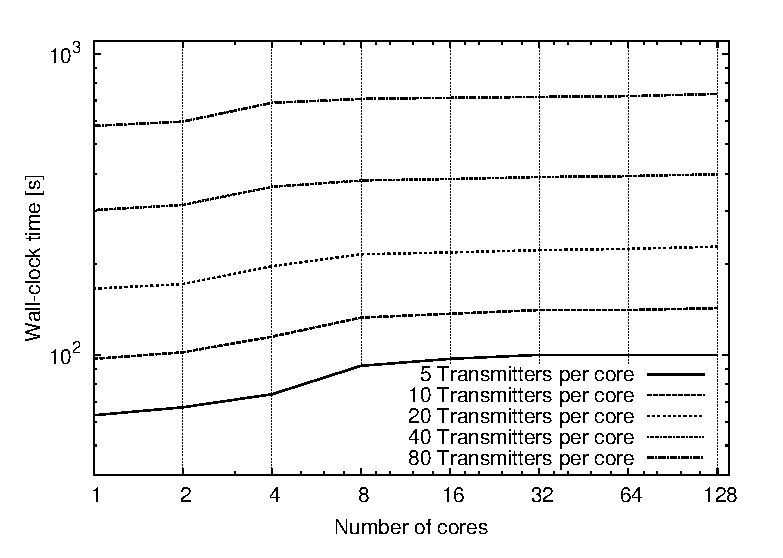
\includegraphics[width=1\columnwidth]{img/weak_scaling-time_plot}

\caption{\textit{\emph{Measured wall-clock time for weak-scalability experiments
as shown in Table \ref{tab:results_weak_scaling}.}}\textit{ }\textit{\emph{Experiments
performed assigned one MPI worker process per available core. The
wall-clock time axis is expressed in base-10 logarithmic scale, whereas
the axis representing the number of cores is expressed in base-2 logarithmic
scale.\label{fig:weak_scalability_time}}}}
\end{figure}


The time measurements observed from the weak-scalability results show
that the wall-clock times do not grow rapidly, especially when the
number of cores is more than 8. Moreover, these times are almost constant
for bigger problem instances, revealing that the achieved level of
scalability gets close-to-linear as the amount of transmitters-per-core
increases. Certainly, the parallel version of PRATO scales especially
well when challenged with a big number of transmitters (10240 for
the biggest instance) over 128 cores. This fact shows PRATO would
be able to calculate the radio coverage prediction for real networks
in a feasible amount of time, since many operational radio networks
have already deployed a comparable number of transmitters, e.g. the
3G network within the Greater London Authority area, in the UK \cite{Number_of_base_stations_in_England}. 

Not being able to achieve perfect weak scalability is due to a number
of factors. Specifically, the overhead time of the serial sections
of the master process grow proportionally with the number of cores,
although the total contribution of this overhead remains low for large
problem sizes. Moreover, the communication overhead grows linearly
with the number of cores used.

To confirm these arguments, we analyze the times of each of the steps
taken by the master process relative to the total processing time.
To this end, we have created plots for three problem instances 5,
20 and 80 transmitters per core, which are shown in \prettyref{fig:weak_scaling-relative_times}.
The relative-processing-time plots follow the formula

\begin{equation}
RT=\frac{t_{\textrm{rd}}+t_{\textrm{ps}}+t_{\textrm{db}}+t_{\textrm{pl}}+t_{\textrm{cp}}}{t_{\textrm{total}}},\label{eq:relative_processing_time}
\end{equation}


\noindent where $t_{\textrm{rd}}$ is the ``Read input data'' wall-clock
time, $t_{\textrm{ps}}$ is the wall-clock time of the ``Dynamic
worker-process spawning'' step, $t_{\textrm{db}}$ is the wall-clock
time of the ``Input data broadcasting'' step, $t_{\textrm{pl}}$
is the wall-clock time of the ``Processing loop'' step, $t_{\textrm{cp}}$
is the wall-clock time of the ``Create final coverage prediction''
step, and $t_{\textrm{total}}$ is the total wall-clock processing
time. For a reference of the different steps taking part of the master
process, see \prettyref{fig:master_process}.

\begin{figure*}[tbh]
\begin{minipage}[t]{0.31\textwidth}%
\centering

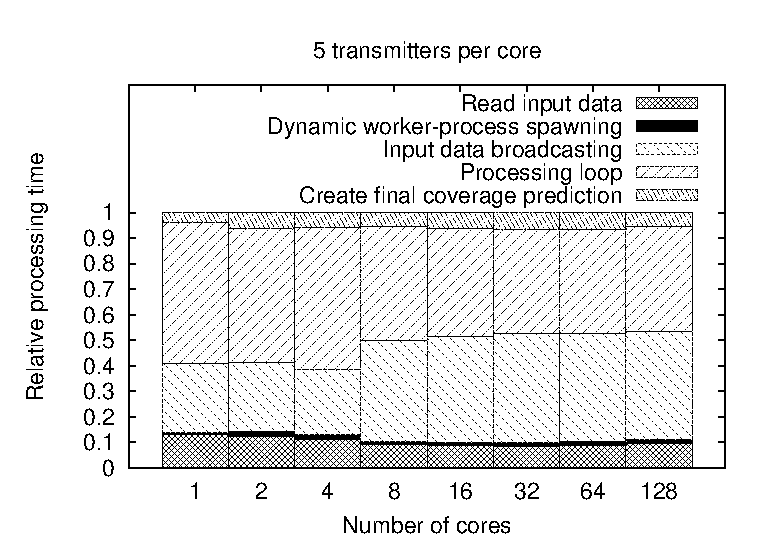
\includegraphics[width=1\columnwidth]{img/weak_scaling_relative_time_plot_5}%
\end{minipage}\qquad{}%
\begin{minipage}[t]{0.31\textwidth}%
\centering

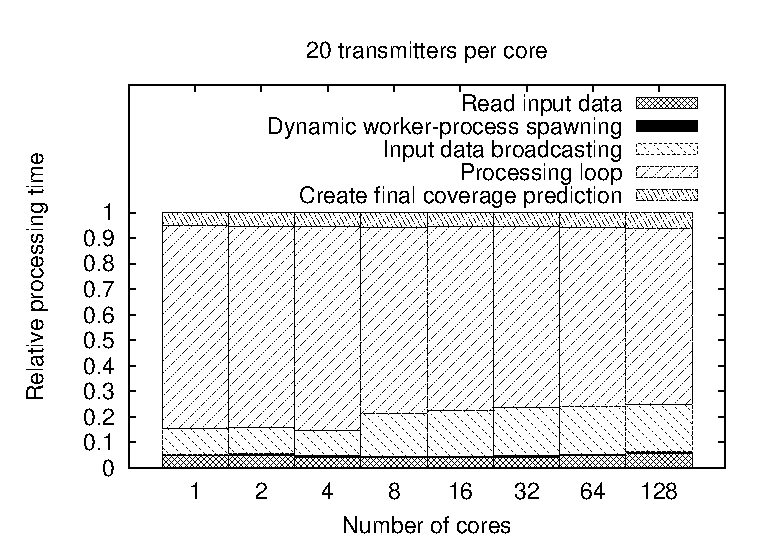
\includegraphics[width=1\columnwidth]{img/weak_scaling_relative_time_plot_20}%
\end{minipage}\qquad{}%
\begin{minipage}[t]{0.31\textwidth}%
\centering

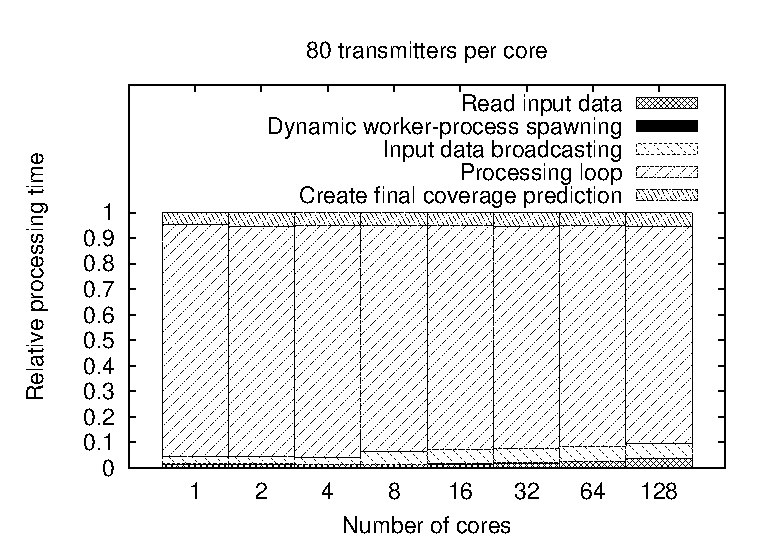
\includegraphics[width=1\columnwidth]{img/weak_scaling_relative_time_plot_80}%
\end{minipage}

\caption{Relative times for the weak-scalability experiments.\emph{ }\textit{\emph{The
relative-processing time axes are expressed in linear scale, whereas
the axes representing the number of cores are expressed in base-2
logarithmic scale.\label{fig:weak_scaling-relative_times}}}}
\end{figure*}


From the relative-times plots, we see that, as we increase the number
of nodes, the largest fraction of the run-time is spent on the parallel
processing of transmitters, which scales notably well for larger problem
instances. The plotted relative times show that there is no dependency
between the relative processing times and the number of cores used,
confirming the good weak-scalability properties noted before. Additionally,
in all three plots we may observe a ``jump'' in the relative time
for the ``Input data broadcasting'' step that takes place when comparing
the result from 4 to 8 cores, i.e. from one to two computing nodes,
as each node hosts ``1 worker per core'' or a total of ``4 workers
per node''. This ``jump'' is due to the use of network communication
when more than one computing node participates in the parallel processing.
In addition, we may also conclude that the network infrastructure
has not been saturated with the data-passing load, since the relative
times for input-data broadcasting do not grow exponentially from 8
cores onward. Regarding the ``Create final coverage prediction''
step, we may see that as we increase the number of cores the relative
times grow proportionally for all three problem sizes.


\subsection{Strong scalability\label{sub:Strong-scalability}}

This set of simulations is meant to analyze the impact of increasing
the number of computing cores for a given problem size, i.e. the number
of transmitters deployed over the target area does not change, while
only the number of cores used is increased. Here we test for the following
number of transmitters: $\{64,128,256,512,1024,2048,4096\}$, and
increase the number of workers per core from 1 to 128 in powers of
2 for each problem size.


\subsubsection{Results and discussion}

The results of the time measurements collected after the simulations
for the strong-scalability experiments are shown in Table \ref{tab:results_strong_scaling}.
All times are expressed in seconds. These wall-clock time measurements
are plotted in \prettyref{fig:strong_scalability_time}, \textit{\emph{where
the time axis is expressed in base-10 logarithmic scale, whereas the
axis representing the number of cores is expressed in base-2 logarithmic
scale.}}

\begin{table}[tbh]
\caption{\textit{\emph{Wall-clock times (in seconds) of the simulation results
for strong scalability.\label{tab:results_strong_scaling}}}}


\centering

{\footnotesize }%
\begin{tabular}{cccccccc}
\cmidrule{2-8} 
 & \multicolumn{7}{c}{{\footnotesize Number of transmitters}}\tabularnewline\addlinespace
\midrule 
{\footnotesize No. cores} & {\footnotesize 64} & {\footnotesize 128} & {\footnotesize 256} & {\footnotesize 512} & {\footnotesize 1024} & {\footnotesize 2048} & {\footnotesize 4096}\tabularnewline
\midrule
{\footnotesize 1} & {\footnotesize 714} & {\footnotesize 1392} & {\footnotesize 2740} & {\footnotesize 5437} & {\footnotesize 10830} & {\footnotesize 21562} & {\footnotesize 43217}\tabularnewline
{\footnotesize 2} & {\footnotesize 386} & {\footnotesize 734} & {\footnotesize 1419} & {\footnotesize 2791} & {\footnotesize 5535} & {\footnotesize 10996} & {\footnotesize 21987}\tabularnewline
{\footnotesize 4} & {\footnotesize 232} & {\footnotesize 408} & {\footnotesize 751} & {\footnotesize 1432} & {\footnotesize 2811} & {\footnotesize 5549} & {\footnotesize 11042}\tabularnewline
{\footnotesize 8} & {\footnotesize 155} & {\footnotesize 242} & {\footnotesize 409} & {\footnotesize 754} & {\footnotesize 1441} & {\footnotesize 2817} & {\footnotesize 5549}\tabularnewline
{\footnotesize 16} & {\footnotesize 113} & {\footnotesize 156} & {\footnotesize 244} & {\footnotesize 414} & {\footnotesize 759} & {\footnotesize 1447} & {\footnotesize 2821}\tabularnewline
{\footnotesize 32} & {\footnotesize 92} & {\footnotesize 114} & {\footnotesize 159} & {\footnotesize 245} & {\footnotesize 414} & {\footnotesize 760} & {\footnotesize 1449}\tabularnewline
{\footnotesize 64} & {\footnotesize 82} & {\footnotesize 94} & {\footnotesize 115} & {\footnotesize 159} & {\footnotesize 245} & {\footnotesize 420} & {\footnotesize 764}\tabularnewline
{\footnotesize 128} & {\footnotesize -} & {\footnotesize 83} & {\footnotesize 94} & {\footnotesize 116} & {\footnotesize 159} & {\footnotesize 248} & {\footnotesize 423}\tabularnewline
\bottomrule
\end{tabular}
\end{table}


\begin{figure}[tbh]
\centering

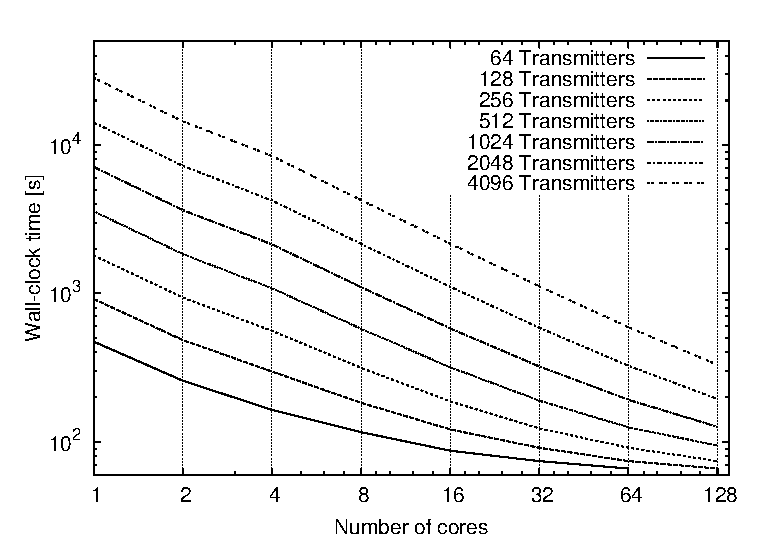
\includegraphics[width=1\columnwidth]{img/strong_scaling-time_plot}

\caption{\textit{\emph{Measured wall-clock time for strong-scalability experiments
as shown in Table \ref{tab:results_strong_scaling}. Experiments performed
assigned one MPI worker process per available core. The wall-clock
time axis is expressed in base-10 logarithmic scale, whereas the axis
representing the number of cores is expressed in base-2 logarithmic
scale.\label{fig:strong_scalability_time}}}}
\end{figure}


The time measurements show that small problem sizes per core have
a relatively large proportion of serial work and communication overhead.
Therefore, the performance deteriorates as the number of transmitters
per core approaches one. It can be observed in \prettyref{fig:strong_scalability_time}
that as we increase the number of transmitters used to solve a given
problem size, the slope of the curve generated by the progression
of wall-clock times tends to a flat line, i.e. as we increase the
number of transmitters there is no reduction in compute time. This
idea is more clearly noted in the test with smaller problem instances,
e.g. 64, 128 and 256 transmitters. In contrast, for the problems with
a number of transmitters larger than 512, the relative contribution
of the non-parallel steps to the wall-clock time is smaller, and a
larger portion of the time is spent on computing the transmitters
coverage in parallel (see Section \ref{sub:Design-parallel} for details
on the steps of PRATO algorithm). A more detailed discussion of the
reasons for the loss of parallel efficiency will be presented towards
the end of this section.

\begin{figure*}[tbh]
\begin{minipage}[t]{0.45\textwidth}%
\centering

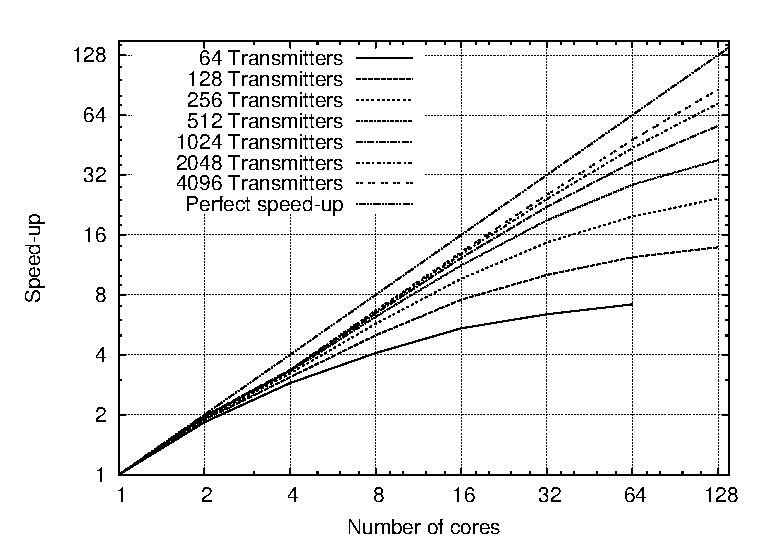
\includegraphics[width=1\columnwidth]{img/strong_scaling-speedup_plot}

\caption{\textit{\emph{Measured speedup for strong-scalability experiments.}}\textit{
}\textit{\emph{The speedup axis is expressed in base-2 logarithmic
scale, whereas the axis representing the number of cores is expressed
in base-2 logarithmic scale.\label{fig:strong_scalability_speedup}}}}
%
\end{minipage}\hfill{}%
\begin{minipage}[t]{0.45\textwidth}%
\centering

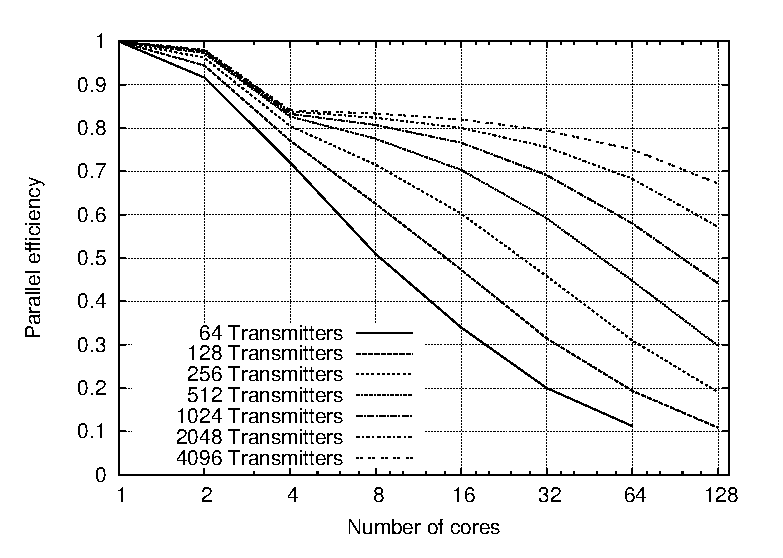
\includegraphics[width=1\columnwidth]{img/strong_scaling-efficiency_plot}

\caption{\textit{\emph{Measured parallel efficiency for strong-scalability
experiments.}}\textit{ }\textit{\emph{The parallel-efficiency axis
is expressed in linear scale, whereas the axis representing the number
of cores is expressed in base-2 logarithmic scale.\label{fig:strong_scalability_efficiency}}}}
%
\end{minipage}
\end{figure*}


In order to observe how well the application scales when compared
against a base case, we have also measured the performance of the
parallel implementation in terms of the speedup, which is defined
as

\begin{equation}
S(NP)=\frac{execution\, time\, for\, base\, case}{execution\, time\, for\, NP\, cores},\label{eq:speedup}
\end{equation}


\noindent where $NP$ is the number of cores executing the worker
processes. As the base case for comparisons we have chosen the parallel
implementation running on only one core and decided against using
the serial implementation. We consider that the serial implementation
is not a good base comparison for the parallel results as it does
not reuse resources between each transmitter coverage calculation
and it does not overlap I/O operations with transmitter computations.
In practice, this means that several concatenated runs of the serial
version would be considerably slower than the parallel but single
worker implementation, because the serial implementation is not able
to use all of the memory bandwidth and computing resources simultaneously.
Therefore such comparison would be entirely biased towards the parallel
implementation, showing super-linear scaling and speedups which would
not be real, as the parallel version is better equipped to make use
of the system resources by means of multiple threads.

Using the speedup metric, linear scaling is achieved when the obtained
speedup is equal to the total number of processors used. However,
it should be noted that perfect speedup is almost never achieved,
due to the existence of serial stages within an algorithm and communication
overheads of the parallel implementation \cite{Cruz_Particle.Flow.Simulation:2010}. 

\prettyref{fig:strong_scalability_speedup} shows the speedup of the
parallel implementation for up to 128 cores (running one worker process
per node), and compares seven different problem sizes with 64, 128,
256, 512, 1024, 2048 and 4096 transmitters deployed over the target
area. The number of transmitters used in these problem sizes are comparable
to several operational radio networks that have already been deployed
in England, e.g. Bedfordshire County with 69 UMTS base stations, Cheshire
County with 132 UMTS base stations, Hampshire County with 227 UMTS
base stations, West Midlands with 414 UMTS base stations, and Greater
London Authority with 1086 UMTS base stations \cite{Number_of_base_stations_in_England}.
Moreover, consider that it is common for a single UMTS base station
to host multiple transmitters. 

We can see that the significant reductions in wall-clock time for
large problem sizes shown in \prettyref{fig:strong_scalability_time}
are directly correlated with the speedup factors shown in \prettyref{fig:strong_scalability_speedup}.

\begin{figure*}[tbh]
\begin{minipage}[t]{0.31\textwidth}%
\centering

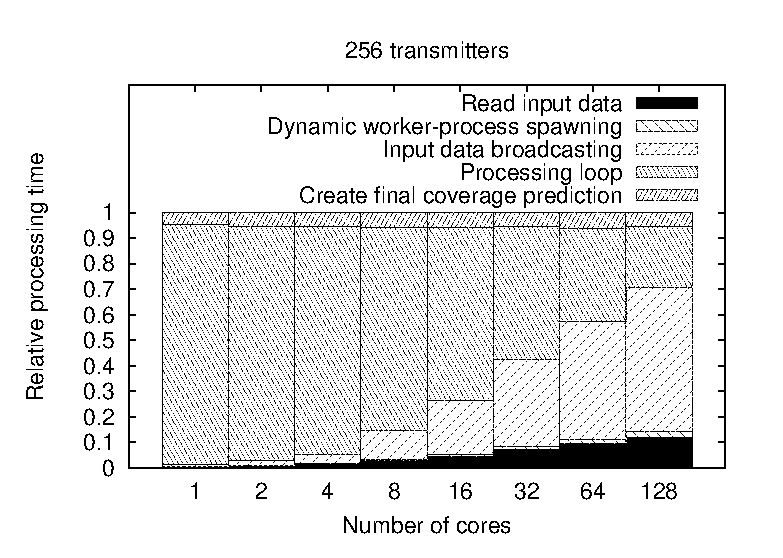
\includegraphics[width=1\columnwidth]{img/strong_scaling-relative_time_plot_256}%
\end{minipage}\qquad{}%
\begin{minipage}[t]{0.31\textwidth}%
\centering

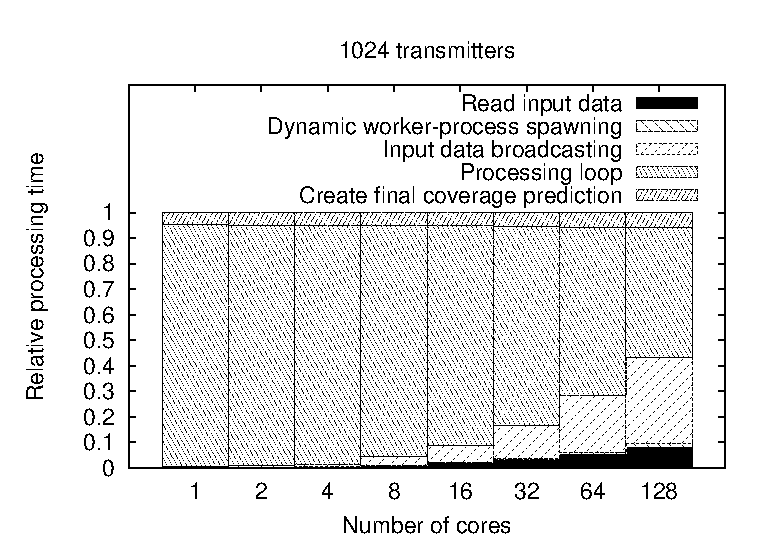
\includegraphics[width=1\columnwidth]{img/strong_scaling-relative_time_plot_1024}%
\end{minipage}\qquad{}%
\begin{minipage}[t]{0.31\textwidth}%
\centering

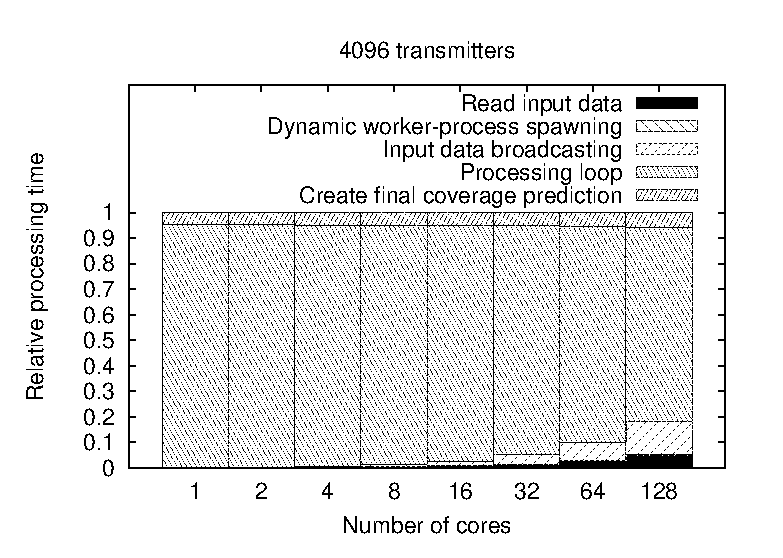
\includegraphics[width=1\columnwidth]{img/strong_scaling-relative_time_plot_4096}%
\end{minipage}

\caption{Relative times for the strong-scalability experiments.\emph{ }\textit{\emph{The
relative-processing time axes are expressed in linear scale, whereas
the axes representing the number of cores are expressed in base-2
logarithmic scale.\label{fig:strong_scaling-relative_times}}}}
\end{figure*}


To study how well PRATO utilizes the available computing resources
we consider the parallel efficiency of the implementation, i.e. how
well the parallel implementation makes use of the available processor
cores. The definition of parallel efficiency is as follows:

\begin{equation}
E(NP)=\frac{S(NP)}{NP},
\end{equation}


\noindent where $S(NP)$ is the speedup as defined in Equation (\ref{eq:speedup}),
and $NP$ is the number of cores executing worker processes. \prettyref{fig:strong_scalability_efficiency}
shows the parallel efficiency of the parallel implementation for different
problem sizes as we increase the number of processing cores. 

The ideal case for a parallel application would be to utilize all
available resources, in which case the parallel efficiency would be
constantly equal to one as we increase the core count. From the plot
in \prettyref{fig:strong_scalability_efficiency}, we may observe
that the efficiency is less than one, hence the computational resources
are under utilized. In accordance to the previous analysis, the under
utilization of the computing resources is more significant for the
smaller problem sizes, where number of assigned transmitters per core
approaches one. This is due to the increased relative influence introduced
by serial and communication overheads, without which the parallel
implementation would not be feasible. On the other hand, the relative
time contribution of the serial and communication overheads is significantly
reduced as the work-load per core increases. Unsurprisingly, these
results confirm what it has previously been suggested during the weak-scaling
analysis, i.e. it is not worth parallelizing small problem instances
over a large number of nodes, since the time reduction due to computations
that make use of the extra parallel resources is surpassed by the
extra parallel initialization and communication overhead.

Similarly as in the weak-scaling test, we study the relative contribution
of each of the steps of the master process as we increase the number
of cores used for a fixed problem size. In this case, we have created
plots for three problem instances, namely 256, 1024 and 4096 transmitters,
which are shown in \prettyref{fig:strong_scaling-relative_times}.
The relative times shown are calculated using the formula depicted
in Equation (\ref{eq:relative_processing_time}).

We may observe the non-parallel steps comprising ``Read input data'',
``Dynamic worker-process spawning'', ``Input data broadcasting''
and ``Final coverage prediction'' contribute with a larger portion
of time as we increase the number of cores, because the total wall-clock
processing time decreases. Additionally, the low parallel efficiency
for small problem sizes, particularly for 256 transmitters (left-most
plot in \prettyref{fig:strong_scaling-relative_times}), is validated
as we see the relative small proportion of the radio-coverage calculation
(``Processing loop'') compared to the serial steps of the process.


\subsection{Load balancing}

In this section, we analyze the level of utilization of the computing
resources available at the computing nodes hosting the worker processes.
Computing-resource utilization is achieved by partitioning the computational
workload and data across all processors. Efficient workload distribution
strategies should be based on the processor speed, memory hierarchy
and communication network \cite{Clarke_Dynamic_load_balancing:2011}.

The parallel implementation of PRATO performs load-balancing using
point-to-point messages (see Section \ref{sub:Master-worker-communication})
between master and worker processes. When a worker process issues
an idle message (see ``Send idle message'' in \prettyref{fig:master_worker_communication}),
the worker process will block until the message arrives to the master
process. A similar situation occurs when the master process signals
a worker back, whether to indicate it to shutdown or to continue working.
Since the process-to-core mapping is one-to-one, blocking messages
typically waste processor cycles on a computing node \cite{Bhandarkar_Adaptive_load_balancing_for_MPI:2001}.
Specifically, we would like to verify the penalties that such synchronization
technique has on the scalability of the parallel implementation.

We evaluate the load empirically \cite{Watts_A_practical_approach_to_dynamic_load_balancing:1998}
by using the following metric as an indicator of the load balancing
among processes:

{\small 
\begin{equation}
LB(NP)=\frac{minimum\, execution\, time\, among\, NP\, cores}{processing\, loop\, time\, of\, master\, process},
\end{equation}
}{\small \par}

\noindent where $NP$ is the number of cores executing worker processes.
Taking the processing-loop time of the master process ensures we measure
the overhead of the message passing during the time while the coverage
prediction is being executed by the workers. This means that the time
measurement is performed excluding the serial parts of the process,
i.e. after the common data have been broadcasted to all worker processes
(``Input data broadcasting'' in \prettyref{fig:master_process}),
until the beginning of the last step (``Create final coverage prediction''
in \prettyref{fig:master_process}).

High performance is achieved when all cores complete their work within
the same time, hence showing a load-balancing factor of one. On the
other hand, lower values indicate disparity between the run times
of the various worker processes sharing the parallel task, thus reflecting
load imbalance.


\subsubsection{Results and discussion}

For this set of experiments, we have chosen the same problem sizes
as for strong scalability in Section \ref{sub:Strong-scalability},
where the coverage predictions are calculated up-to 128 cores, running
on 32 computing nodes.

\begin{figure}[tbh]
\centering

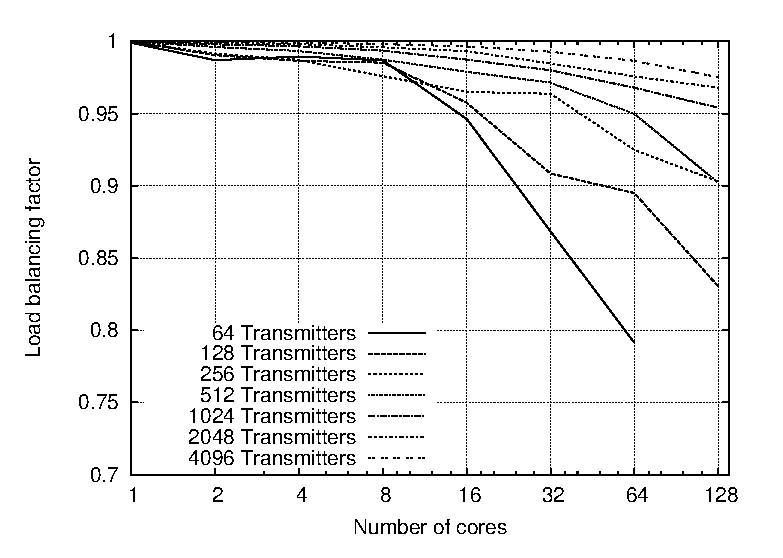
\includegraphics[width=1\columnwidth]{img/strong_scaling-load_balancing_plot}

\caption{\textit{\emph{Load balancing among worker processes.\label{fig:load_balancing}}}}
\end{figure}


From the plot shown in \prettyref{fig:load_balancing}, it is clear
that the influence of the message-passing overhead over the processing
time is inversely proportional to the amount of work each worker process
receives. Additionally, for the biggest problem instances (1024, 2048
and 4096 transmitters), parallel-process execution times are within
95\% of a perfect load-balancing factor, and within 90\% for problem
sizes with 256 and 512 transmitters, showing a very good performance
of the dynamic task assignment, driven by our message-passing technique.
For problem instances of 64 and 128 transmitters, the parallel-process
times are within 80\% of the perfect load balancing, showing that,
as the number of transmitters per core approaches to one, latencies
introduced by several hardware and OS-specific factors (e.g. TurboBoost,
process affinity, etc.) are influential over the total process time.
Particularly, message-passing is not able to compensate these latencies
as it is executed only once per worker process.

It is worth pointing out that the very good load-balancing factors
shown here are not only merit of the message-passing technique. The
result dumping of partial path-loss predictions, performed by the
worker processes in a separate thread into an external database server,
prevents data synchronization from occurring at each iteration of
the parallel process, consequently improving the load-balancing factors
significantly.


\section{Related work \label{sec:Related-work}}

As it has been mentioned before, the reference implementation for
PRATO is the work done by Hrovat et al. \cite{Ozimek_Open.source.radio.coverage.prediction:2010}.
The reported results show a comparable quality to those of a professional
radio-planning tool. Since the results of the conducted comparison
tests showed identical results between PRATO and this work, we may
conclude that PRATO reaches solutions of comparable quality to those
of a professional tool. However, a performance comparison with this
work has not been performed, because it only deals with serial implementations. 

A different example of a GIS-based open-source radio planning tool,
called Q-Rap, has been presented in \cite{QRap}. Developed by the
University of Pretoria and the Meraka Institute of South Africa, the
software was made publicly available in May 2010. Its design is geared
towards an end-user tool with a graphical user interface, not appropriate
for big batch jobs involving thousands of transmitters, or even parallel
job execution. It is implemented as a plug-in for the Quantum GIS
(QGIS) open source system \cite{QuantumGIS}.

The task-parallelization problem within the GRASS environment has
been addressed by several authors in different works. Campos et al.
\cite{Campos_Parallel_modelling_in_GIS:2012} present a collection
of GRASS modules for watershed analysis. Their work concentrates on
different ways of slicing raster maps to take advantage of a potential
MPI implementation, but there are no guidelines for work replication.
Moreover, the hardware specification, on which the experiments have
been run, is missing, making it very difficult to build upon this
work.

On the field of high-performance computing, Akhter et al. \cite{Akhter_Porting_GRASS_raster_module_to_distributed_computing:2007}
have presented implementation examples of a GRASS raster module, used
to process vegetation indexes for satellite images, for MPI and Ninf-G
environments. The main drawback with their methodology is the compulsory
use of GRASS libraries in all the computing nodes that take part in
the parallel calculation, making them more difficult to setup. Moreover,
the authors explicitly acknowledge a limitation in the performance
of their MPI implementation for big processing jobs. The restriction
appears due to the computing nodes being fixed to a specific range,
since the input data are equally distributed among worker processes,
creating an obstacle for load balancing in heterogeneous environments.
It is worth pointing out that in the parallel implementation of PRATO
we specifically address this problem with our message-passing technique.

Similarly, Huang et al. \cite{Huang_Cluster_based_parallel_GIS:2011}
use the parallel inverse distance weighting interpolation algorithm
as a parallel-pattern example. Although it is not explicitly noted,
it can be concluded that the computing nodes make use of the GRASS
environment, again making them more difficult to setup. Moreover,
since the amount of work is evenly distributed among all processes
(including the master one), their approach would also show decreased
efficiency in heterogeneous environments.


\section{Conclusion}

We have presented the design and implementation of PRATO, a parallel
radio-coverage prediction tool for GRASS GIS. Extensive simulations
were performed in the DEGIMA computer cluster of the Nagasaki Advanced
Computing Center. The results have been analyzed to determine the
level of scalability of the implementation, as well as the impact
of the introduced patterns for parallel algorithm design within GRASS
GIS.

The conducted analysis shows that PRATO is able to calculate the radio-coverage
prediction of real-world mobile networks in a reduced amount of time
with a high scalability level. The promising results also show the
great potential of our approach to parallelize other time-consuming
tasks for GRASS GIS, although this point still has to be fully demonstrated.
Particularly, the gathered results suggest that our approach would
be also beneficial in the area of mobile network optimization, where
thousands of simulations take part of the evaluation step during an
optimization process. Still, further research is needed on how this
method may be fully exploited.

Nevertheless, as PRATO is a free and open-source software project,
it can be readily modified and extended to support, for example, other
propagation models and post-processing algorithms. This characteristic
defines a clear advantage when compared to commercial and closed-source
tools.


\section*{Acknowledgments}

This project was co-financed by the European Union, through the European
Social Fund. Hamada acknowledges support from the Japan Society for
the Promotion of Science (JSPS) through its Funding Program for World-leading
Innovative R\&D on Science and Technology (First Program).

{\footnotesize \bibliographystyle{ieeetr}
\bibliography{manuscript}
}{\footnotesize \par}

\begin{IEEEbiographynophoto}{Lucas Benedi\v{c}i\v{c}} received his
M.Sc. in computer sciences from the University of Primorska, Koper,
Slovenia, in 2009. He is a Ph.D. candidate at the Jo\v{z}ef Stefan
International Postgraduate School, currently holding a position in
the Research and Development Department at Telekom Slovenije, d.d.,
in Ljubljana, Slovenia. His research interests include parallel algorithms,
high-performance computing, GPGPU, and combinatorial optimization
applied to mobile networks. More information is available at \href{http://csd.ijs.si/benedicic/}{http://csd.ijs.si/benedicic/}.

\end{IEEEbiographynophoto}

\begin{IEEEbiographynophoto}{Felipe A. Cruz} was born in Chile in
1982. He received the B.~Eng., P.~Eng, and M.Sc. degree in informatic
engineering from the Universidad T\'{e}cnica Federico Santa Mar\'{i}a,
Valpara\'{i}so, Chile, in 2004, 2006, and 2007, respectively. He
received the Ph.D. degree in mathematics from the University of Bristol,
U.K., in 2011. He is currently a postdoctoral fellow at the Nagasaki
Advanced Computing Center at Nagasaki University, Japan.

\end{IEEEbiographynophoto}\begin{IEEEbiographynophoto}{Tsuyoshi Hamada}
received his Ph.D. in 2006 from the University of Tokyo. From 2006
to 2008 he was a Special Postdoctoral Researcher at RIKEN. In 2008
he became an Assistant Professor at Nagasaki University, and was promoted
to Associate Professor in 2010. With his work on massively parallel
architectures he was awarded the Gordon Bell prize for prize/performance
in 2009 and a Gordon Bell prize Honorable mention in 2010. He is currently
the deputy director of the Nagasaki Advanced Computing Center at Nagasaki
University, Japan.

\end{IEEEbiographynophoto}

\begin{IEEEbiographynophoto}{Peter Koro\v{s}ec} received his Ph.D.
from the Jo\v{z}ef Stefan International Postgraduate School, Ljubljana,
Slovenia, in 2006. Since winter 2002 he has been a researcher at the
Jo\v{z}ef Stefan Institute, Ljubljana, Slovenia. He is presently
a researcher at the Computer Systems department and an assistant professor
at the University of Primorska, Faculty of Mathematics, Natural Sciences
and Information Technologies Koper, Koper, Slovenia. His research
interests include combinatorial and numerical optimization with modern
metaheuristics in parallel and distributed computing. More information
about his work can be found at \href{http://csd.ijs.si/korosec/}{http://csd.ijs.si/korosec/}.

\end{IEEEbiographynophoto}
\end{document}
